% ABCSS 2026 submission, IEEE BigData 2026 workshop. Single-blind, so the
% author block is filled in. Limit: 10 pages including references.
\documentclass[conference]{IEEEtran}
\IEEEoverridecommandlockouts

\usepackage{cite}
\usepackage{amsmath,amssymb,amsfonts}
\usepackage{amsthm}
\usepackage{graphicx}
\usepackage{booktabs}
\usepackage{nicefrac}
\usepackage{url}
\usepackage{xcolor}
\usepackage[hidelinks]{hyperref}

\theoremstyle{plain}
\newtheorem{theorem}{Theorem}
\newtheorem{lemma}[theorem]{Lemma}
\newtheorem{corollary}[theorem]{Corollary}
\newtheorem{proposition}[theorem]{Proposition}

\newcommand{\Neff}{N_{\mathrm{eff}}}
\newcommand{\mN}{m_N}
\newcommand{\lmax}{\lambda_{\max}}
\newcommand{\one}{\mathbf{1}}

\begin{document}

\title{Herd Immunity and Learning Externalities in\\ Markets of Shared Foundation Models}

\author{%
\IEEEauthorblockN{Vignesh Nagarajan}
\IEEEauthorblockA{Texas A\&M University\\
College Station, TX, USA\\
vigneshn26@tamu.edu}
\and
\IEEEauthorblockN{Shriraghav Ashok}
\IEEEauthorblockA{University of California, Berkeley\\
Berkeley, CA, USA\\
sashok24@berkeley.edu}
}

\maketitle

\begin{abstract}
% TODO
\end{abstract}

\begin{IEEEkeywords}
% TODO
\end{IEEEkeywords}

\section{Introduction}
\label{sec:intro}

Picture fifty dealers quoting the same bonds. Each one retrains its pricing model on the order flow it saw since the last retraining, and each one, tested on its own, is fine: replay its own history and it settles down. Put the fifty in one market and the market can still blow up. The flow a dealer sees depends on how the other forty-nine priced, so every retraining changes what everyone else learns from next. None of the fifty models accounts for that.

We call this a \emph{learning externality}. The broader idea, that sensible individual behavior can add up to collective fragility, is old. Banks that each diversify optimally end up holding the same portfolios and fail together \cite{beale2011,wagner2010}. Quantitative funds running similar strategies unwound together in August 2007, and no single fund's risk report showed the crowding \cite{khandani2007}. What is new is that the agents now learn, and more and more of them learn from the same place. Firms that fine-tune one vendor's foundation model make correlated errors \cite{kim2025}. We show that they also push the market in correlated directions, and that this, rather than the number of firms, is what decides whether the market is stable.

The tool people use today looks at one model at a time. A learner whose deployment reshapes its own data converges under repeated retraining when a single number, its performative modulus $m$, stays below one \cite{perdomo2020}. Certify $m<1$ and the loop is safe. In a market that certificate is not enough. The quantity that matters is a market-level number we call the \emph{feedback reproduction number} $\mN$, the factor by which a shared disturbance grows per round of retraining. The market converges exactly when $\mN<1$, and $\mN$ depends on how many independent models sit under the market. Fifty firms built on one vendor's model behave like one learner fifty times larger. Fifty firms built on fifty unrelated models behave like one firm.

The result we like best started as a mistake. Our first version of the herd-immunity result took a limit in which correction is perfect, and it produced a clean threshold: correct enough firms and the market is safe. When we checked that threshold against the exact spectral radius on random markets, it was wrong in the dangerous direction. It called $11.8\%$ of configurations stable that are unstable at every finite correction strength. Working out the exact threshold turned up a formula epidemiologists already use, the coverage a population needs when the vaccine is imperfect \cite{anderson1985,fine2011}, together with an efficacy below which no coverage is enough. The clean limit is still in the paper, but as a corollary with its error direction stated.

\subsection*{Contributions}
\begin{enumerate}
\item \emph{Effective crowding.} The stability of a market of retraining firms is governed by $\mN=\Neff m_1$, where $\Neff$ depends on the leading eigenvalue of a correlation matrix of the firms' response directions (Section~\ref{sec:crowding}). Diversity indices built on mean similarity can call an unstable market safe.
\item \emph{Herd immunity.} An exact stability threshold for a market mixing corrected and uncorrected firms, which reduces to the imperfect-vaccine coverage law and implies a critical efficacy. Correction and model diversity substitute for each other along a frontier we compute (Section~\ref{sec:herd}).
\item \emph{Cadence and a tax.} Retraining in smaller steps helps only below a critical crowding level, and a Pigouvian fee prices the externality. Without the fee, every market of two or more firms adapts too aggressively (Section~\ref{sec:levers}).
\item \emph{Honest evidence.} Every numerical check carries its status. One is measured in an order-flow market, and the rest confirm the formulas against the model they came from. Full proofs, code and 542 numerical certificates are public \cite{price2026}.
\end{enumerate}

\subsection*{What this paper is not}
It is not an empirical study of a deployed market. Our one measured result comes from an order-flow simulator we built for earlier work \cite{reflex2026}. We have not yet measured the key eigenvalue on any real set of deployed models, and Section~\ref{sec:conclusion} says how we would. What we offer is the quantity a supervisor would need to measure and the three instruments that act on it.

\section{Related work}
\label{sec:related}

\subsection{Collective behavior and contagion}
Threshold models explain how a behavior spreads once enough others have adopted it \cite{granovetter1978}, and informational cascades explain why people rationally copy their predecessors and why the resulting consensus is fragile \cite{bikhchandani1992}. Both are about people imitating people. In our setting nobody imitates anyone. Firms become correlated because they learn from shared data through shared models. The epidemiological link is an identity rather than an analogy: $R_0$ is defined as the spectral radius of a next-generation operator \cite{diekmann1990}, $\mN$ is the spectral radius of a linearized retraining operator, and so the two thresholds are the same statement. That is why the vaccination results carry over with their refinements, including the imperfect-vaccine law. Heterogeneous contact structure famously changes epidemic thresholds \cite{pastorsatorras2001}. Here the analogous structure is the alignment matrix.

\subsection{Algorithmic monoculture}
When many firms adopt one algorithm, welfare can fall even if that algorithm is the better one, because independent errors stop cancelling \cite{kleinberg2021}. Shared models also concentrate harm on the same individuals \cite{bommasani2022}, and a shared evaluation algorithm changes outcomes in matching markets \cite{peng2024}. These results describe a market at rest. None gives a stability boundary, so a market can look fine at equilibrium and still be one retraining away from diverging.

\subsection{Performative prediction with many learners}
Performative prediction studies learners whose deployments shift their own data \cite{perdomo2020}. With several learners in one environment, convergence conditions exist that bound scalar sensitivities against curvature \cite{narang2023}, and in the fully aligned case, increasing learning rates and agent counts can drive the dynamics into chaos \cite{piliouras2023}. Our condition bounds a spectral radius instead, and Proposition~\ref{prop:witness} shows two markets that agree on every scalar such a criterion reads but differ in stability. We also compose two single-learner tools with the market: lazy deployment, where a learner takes a few gradient steps per round \cite{mendlerdunner2020}, and feedback-aware updates that correct for the learner's own influence \cite{izzo2021,miller2021}.

\subsection{Systemic risk and random matrices}
The largest eigenvalue of a correlation matrix as the weight of a common market mode is standard in econophysics \cite{laloux1999,plerou2002}. We compute it from a different matrix, response directions instead of returns, and it enters a stability condition rather than a portfolio. Reading economic conditions from public text works through an exogenous channel \cite{pebsa2024}. The supervisory estimator in Section~\ref{sec:conclusion} reads an endogenous one, and its signal gets stronger as the market approaches the boundary it is watching for.

\section{A market of retraining firms}
\label{sec:setup}

\subsection{The symmetric market}
Start with $N$ dealers quoting the same instruments and drawing on one pool of informed order flow. When one dealer tightens its quotes, more toxic flow reaches every dealer, in proportion to a spillover $\kappa\in[0,1]$. Each dealer retrains periodically on the flow it has seen, and on its own it is stable exactly when its performative modulus satisfies $m_1<1$. Here $m_1=\varepsilon\beta/\gamma$, where $\varepsilon$ is how strongly the flow responds to the dealer's quotes, $\beta$ is how sensitive its loss is to that response, and $\gamma$ is the curvature of its objective \cite{perdomo2020}.

Linearize the joint retraining map around the market's equilibrium. Its Jacobian is $J=-m_1[(1-\kappa)I+\kappa\one\one^{\top}]$, and its largest mode, the one where all dealers move together, has size $m_1(1+\kappa(N-1))$. The market therefore goes unstable at a response strength $1+\kappa(N-1)$ times smaller than any single dealer can tolerate. This law comes from our earlier work \cite{reflex2026}, and Section~\ref{sec:evidence} measures it. Everything below replaces one object in it: the all-ones matrix $\one\one^{\top}$, which says every dealer pushes the flow in the same direction.

The economics is worth a sentence. A price change is a transfer between parties. Changing the data a competitor learns from changes its forecasting technology, which is a real efficiency loss, a technological externality in the classical sense \cite{buchanan1962}. And nothing in dealer A's validation data contains dealer B, so no single-model test can see it.

\subsection{Response directions and the alignment matrix}
In a real market firms do not all push the same way. Give firm $i$ a response Jacobian $E_i\in\mathbb{R}^{d\times d}$, describing how its deployment reshapes the flow it faces. The \emph{alignment matrix} $R$ has entries
\begin{equation}
r_{ij}=\frac{\langle \mathrm{vec}\,E_i,\mathrm{vec}\,E_j\rangle}{\|E_i\|_F\,\|E_j\|_F},
\end{equation}
the correlation between two firms' feedback directions. It is positive semidefinite with ones on the diagonal, like a correlation matrix of returns, but it measures something different: whether two firms' models distort the market the same way.

We work under four standing assumptions. (A1) Stability statements linearize the joint map at equilibrium, and the simulator serves as the nonlinear check. (A2) Firms have equal moduli $m_i=m_1$; unequal moduli give two-sided bounds. (A3) Firms retrain on a common clock. (A4) Firms couple through one pool with scalar spillover $\kappa$.

\begin{lemma}[Reduction]
\label{lem:reduction}
Suppose each firm's deviation from equilibrium is a scalar $x_i$ along its own unit response direction, all $\|E_i\|_F$ are equal to $\varepsilon$, each firm feels its own distortion in full and a competitor's with weight $\kappa$, both measured along its own direction, and each firm best-responds under a $\gamma$-strongly convex objective with sensitivity $\beta$. Then the joint retraining map is linear with Jacobian
\begin{equation}
\label{eq:reduction}
J=-m_1\bigl[(1-\kappa)I+\kappa R\bigr].
\end{equation}
\end{lemma}

The proof is two lines. The pool carries the total distortion $\sum_j x_jE_j$, firm $i$ reads it along its own direction, and the inner products are $\varepsilon r_{ij}$. The hypothesis that firms read the pool only along their own direction is literal in a dealer market. A dealer sees order flow only where it quotes. Flow that a competitor's repricing pushes into instruments the dealer does not trade never reaches its training set, however large it is. That is why two firms perturbing the market in orthogonal directions do not affect each other, and why $R$ shows up at all.

\section{Effective crowding}
\label{sec:crowding}

Counting firms gives the wrong answer. The right count is the leading eigenvalue $\lmax(R)$, which runs from $1$, when all response directions are orthogonal, to $N$, when they all coincide.

\begin{theorem}[Alignment sets the reproduction number]
\label{thm:alignment}
Under (A1)--(A4) and Lemma~\ref{lem:reduction}, the market's spectral radius is
\begin{equation}
\mN=\Neff\,m_1,\qquad \Neff=1+\kappa\bigl(\lmax(R)-1\bigr),
\end{equation}
and the market is stable if and only if $\mN<1$.
\end{theorem}

In words: a market behaves like $\Neff$ copies of one firm, and $\Neff$ counts independent models, not firms.

Four cases make this concrete. If every firm shares one model, $R=\one\one^{\top}$ and we recover the symmetric law $\Neff=1+\kappa(N-1)$. If every firm's direction is orthogonal to every other, $R=I$ and $\Neff=1$: a hundred firms pushing in a hundred unrelated directions are dynamically one firm. If each firm's response is a share $s$ from a common foundation model, vendor or pretraining corpus and $1-s$ its own, alignments concentrate at $s$ and $\Neff\to1+\kappa s(N-1)$. And in every case $\Neff\ge1$, so interaction never makes a market more stable than its members are alone.

\begin{proposition}[Scalars are not enough]
\label{prop:witness}
Fix $N\ge2$, $\kappa\in(0,1]$ and $1/(1+\kappa(N-1))<m_1<1$. The markets with $R=I$ and $R=\one\one^{\top}$ share $\varepsilon$, $\beta$, $\gamma$, $m_1$ and $\kappa$, yet the first is stable and the second is not.
\end{proposition}

At $N=20$, $\kappa=0.8$ and $m_1=0.15$, the orthogonal market has $\mN=0.15$ and the monoculture has $\mN=2.43$. One converges and the other diverges, and no Lipschitz constant or curvature bound in either model tells them apart. The alignment matrix does.

\subsection{Provenance, not concentration}
The supply-chain form $\mN=m_1(1+\kappa s(N-1))$ says the stability condition is driven by where the models come from. A competition regulator looks at concentration. Fifty equal-share firms have the lowest possible Herfindahl index \cite{hirschman1964} and look perfectly competitive. If all fifty fine-tune one vendor's model, they are dynamically a monoculture. Error correlation across more than 350 hosted language models is substantial and clusters within providers \cite{kim2025}, so the premise of the decomposition is already visible in deployed systems. Fig.~\ref{fig:phase} shows the stability boundary in the $(N,s)$ plane.

\begin{figure}[!t]
\centering
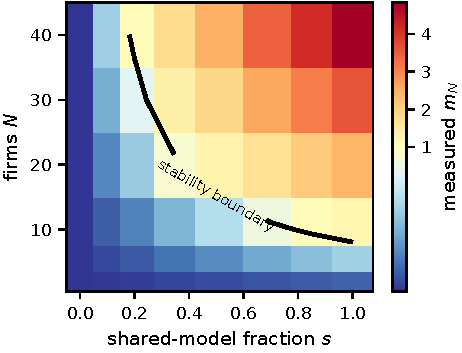
\includegraphics[width=0.82\columnwidth]{figures/fig_phase.pdf}
\caption{Measured $\mN$ across 48 cells of firm count $N$ and shared-model fraction $s$, with the predicted stability boundary. The reference environment agrees with Theorem~\ref{thm:alignment} in every cell to within $7.1\times10^{-15}$ (Section~\ref{sec:evidence}).}
\label{fig:phase}
\end{figure}

\subsection{Why mean similarity fails}
A natural diversity index averages pairwise similarity. The average understates \emph{clustered} alignment. Take ten firms, three tightly aligned and the rest orthogonal, with $\kappa=0.8$. Then $\Neff=2.60$, against $1.48$ for a uniform configuration with the same mean. At $m_1=0.5$ the clustered market has $\mN=1.30$ and diverges, while the mean-based index reports $0.74$ and calls it safe with room to spare. The error only ever runs one way: $\Neff\ge1+\kappa(N-1)\bar r$ for every $R$, so a mean-based index never overstates risk. It can only miss it.

\section{Herd immunity}
\label{sec:herd}

Slowing down is something a firm can do on its own (Section~\ref{sec:levers}). Correction is different: it only works if enough firms do it. A \emph{corrected} firm runs a feedback-aware update that accounts for its own influence on the data \cite{izzo2021,miller2021}. Its modulus shrinks by a factor $\theta=\gamma/\gamma_{\mathrm{PO}}<1$, where $\gamma_{\mathrm{PO}}$ is the curvature of the objective once the feedback is priced in. Correction changes how hard a firm pushes, not which way, so $R$ is unchanged.

Consider a market of $N_b$ uncorrected (``blind'') firms and $N_c=N-N_b$ corrected ones, with corrected fraction $\rho_c=N_c/N$.

\begin{theorem}[Mixed-market stability]
\label{thm:mixed}
Under (A1)--(A4) with supply-chain alignment $s$ and $1\le N_b\le N-1$, write $\tilde\kappa=\kappa s$. The spectral radius is the larger root
\begin{equation}
\rho(J)=\tfrac12\Bigl(P+\sqrt{P^2-4Q}\Bigr),
\end{equation}
where $P=(1-\tilde\kappa)m_1(1+\theta)+\tilde\kappa m_1(N_b+\theta N_c)$ and $Q=\theta m_1^2(1-\tilde\kappa)\Neff$.
\end{theorem}

The radius comes from a secular equation, a diagonal matrix plus a rank-one term, which with two correction levels collapses to a quadratic. $\Neff$ sits inside $Q$, so the mixed market inherits the crowding of Section~\ref{sec:crowding} directly.

\subsection{The limit that was too optimistic}
Let correction become perfect, $\gamma_{\mathrm{PO}}\to\infty$. Then only blind firms can sustain an unstable cycle, and the market is stable when $N_b<1+(1/m_1-1)/(\kappa s)$. This is the clean threshold we started with, and it errs in the wrong direction. The radius is nondecreasing in $\theta$ (Perron--Frobenius, on a nonnegative matrix), so the perfect-correction limit understates it. On random draws it calls 2157 of 18313 configurations stable that are unstable at every finite correction strength, $11.8\%$ with exact $95\%$ interval $[11.3\%,12.3\%]$. The same monotonicity gives the reassuring half: correcting a firm never destabilizes the market.

\subsection{The imperfect-vaccine law}
In the corner $\kappa=s=1$ the perfect-correction limit reads $\rho_c^*=1-1/\mN$. This is exactly the herd-immunity threshold $1-1/R_0$, with $\mN$ playing the role of the reproduction number. A market of ten firms at $\mN=2.5$ needs six of them corrected, if correction is perfect. It is not, and at the same corner the exact condition solves to
\begin{equation}
\rho_c^*(e)=\frac{1-1/\mN}{e},\qquad e=1-\frac{\gamma}{\gamma_{\mathrm{PO}}},
\end{equation}
where $e$ is the \emph{efficacy} of correction. This is the standard coverage requirement for an imperfect vaccine \cite{anderson1985,fine2011}. The clean law assumes homogeneous mixing, and the corner $\kappa=s=1$ is the market's version of that assumption.

\begin{corollary}[Critical efficacy]
\label{cor:efficacy}
No corrected fraction stabilizes the market when $\theta>1/\mN$. Correction is a usable lever only if $\gamma_{\mathrm{PO}}/\gamma>\mN$.
\end{corollary}

At $\mN=2.5$, correction must improve curvature by more than a factor of $2.5$ or it cannot save the market at any coverage. Fig.~\ref{fig:herd} shows the thresholds moving right as efficacy falls.

\begin{figure}[!t]
\centering
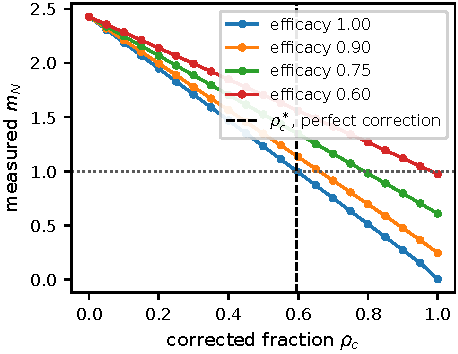
\includegraphics[width=0.82\columnwidth]{figures/fig_herd.pdf}
\caption{Market modulus $\mN$ against corrected fraction at $N=20$, $m_1=0.15$, $\kappa=0.8$, $s=1$, for four efficacies. The dashed line is the perfect-correction threshold. The gap between it and each crossing is the error Section~\ref{sec:herd} describes, not noise.}
\label{fig:herd}
\end{figure}

\subsection{Diversity as a substitute}
The required coverage $\rho_c^*$ rises with $s$ wherever it is positive, so a market can reach stability along either axis. At $N=20$, $m_1=0.15$ and $\kappa=0.8$, a monoculture needs $12$ corrected firms, a market at $s=0.5$ needs five, and a market at $s=0.2$ needs none.

Both remedies are public goods. A corrected firm pays for its correction and everyone shares the stability. A firm that picks an idiosyncratic model pays for that choice and supplies stability to competitors for free. So the market under-supplies both \cite{bergstrom1986}, and the trade-off between them is a trade-off between two goods that are each too scarce.

\section{Two more levers: cadence and a tax}
\label{sec:levers}
% TODO

\section{Evidence}
\label{sec:evidence}
% TODO

\section{Limitations and conclusion}
\label{sec:conclusion}
% TODO

\bibliographystyle{IEEEtran}
\bibliography{references}

\end{document}
